% Options for packages loaded elsewhere
\PassOptionsToPackage{unicode}{hyperref}
\PassOptionsToPackage{hyphens}{url}
%
\documentclass[
]{article}
\usepackage{amsmath,amssymb}
\usepackage{iftex}
\ifPDFTeX
  \usepackage[T1]{fontenc}
  \usepackage[utf8]{inputenc}
  \usepackage{textcomp} % provide euro and other symbols
\else % if luatex or xetex
  \usepackage{unicode-math} % this also loads fontspec
  \defaultfontfeatures{Scale=MatchLowercase}
  \defaultfontfeatures[\rmfamily]{Ligatures=TeX,Scale=1}
\fi
\usepackage{lmodern}
\ifPDFTeX\else
  % xetex/luatex font selection
\fi
% Use upquote if available, for straight quotes in verbatim environments
\IfFileExists{upquote.sty}{\usepackage{upquote}}{}
\IfFileExists{microtype.sty}{% use microtype if available
  \usepackage[]{microtype}
  \UseMicrotypeSet[protrusion]{basicmath} % disable protrusion for tt fonts
}{}
\makeatletter
\@ifundefined{KOMAClassName}{% if non-KOMA class
  \IfFileExists{parskip.sty}{%
    \usepackage{parskip}
  }{% else
    \setlength{\parindent}{0pt}
    \setlength{\parskip}{6pt plus 2pt minus 1pt}}
}{% if KOMA class
  \KOMAoptions{parskip=half}}
\makeatother
\usepackage{xcolor}
\usepackage[margin=1in]{geometry}
\usepackage{color}
\usepackage{fancyvrb}
\newcommand{\VerbBar}{|}
\newcommand{\VERB}{\Verb[commandchars=\\\{\}]}
\DefineVerbatimEnvironment{Highlighting}{Verbatim}{commandchars=\\\{\}}
% Add ',fontsize=\small' for more characters per line
\usepackage{framed}
\definecolor{shadecolor}{RGB}{248,248,248}
\newenvironment{Shaded}{\begin{snugshade}}{\end{snugshade}}
\newcommand{\AlertTok}[1]{\textcolor[rgb]{0.94,0.16,0.16}{#1}}
\newcommand{\AnnotationTok}[1]{\textcolor[rgb]{0.56,0.35,0.01}{\textbf{\textit{#1}}}}
\newcommand{\AttributeTok}[1]{\textcolor[rgb]{0.13,0.29,0.53}{#1}}
\newcommand{\BaseNTok}[1]{\textcolor[rgb]{0.00,0.00,0.81}{#1}}
\newcommand{\BuiltInTok}[1]{#1}
\newcommand{\CharTok}[1]{\textcolor[rgb]{0.31,0.60,0.02}{#1}}
\newcommand{\CommentTok}[1]{\textcolor[rgb]{0.56,0.35,0.01}{\textit{#1}}}
\newcommand{\CommentVarTok}[1]{\textcolor[rgb]{0.56,0.35,0.01}{\textbf{\textit{#1}}}}
\newcommand{\ConstantTok}[1]{\textcolor[rgb]{0.56,0.35,0.01}{#1}}
\newcommand{\ControlFlowTok}[1]{\textcolor[rgb]{0.13,0.29,0.53}{\textbf{#1}}}
\newcommand{\DataTypeTok}[1]{\textcolor[rgb]{0.13,0.29,0.53}{#1}}
\newcommand{\DecValTok}[1]{\textcolor[rgb]{0.00,0.00,0.81}{#1}}
\newcommand{\DocumentationTok}[1]{\textcolor[rgb]{0.56,0.35,0.01}{\textbf{\textit{#1}}}}
\newcommand{\ErrorTok}[1]{\textcolor[rgb]{0.64,0.00,0.00}{\textbf{#1}}}
\newcommand{\ExtensionTok}[1]{#1}
\newcommand{\FloatTok}[1]{\textcolor[rgb]{0.00,0.00,0.81}{#1}}
\newcommand{\FunctionTok}[1]{\textcolor[rgb]{0.13,0.29,0.53}{\textbf{#1}}}
\newcommand{\ImportTok}[1]{#1}
\newcommand{\InformationTok}[1]{\textcolor[rgb]{0.56,0.35,0.01}{\textbf{\textit{#1}}}}
\newcommand{\KeywordTok}[1]{\textcolor[rgb]{0.13,0.29,0.53}{\textbf{#1}}}
\newcommand{\NormalTok}[1]{#1}
\newcommand{\OperatorTok}[1]{\textcolor[rgb]{0.81,0.36,0.00}{\textbf{#1}}}
\newcommand{\OtherTok}[1]{\textcolor[rgb]{0.56,0.35,0.01}{#1}}
\newcommand{\PreprocessorTok}[1]{\textcolor[rgb]{0.56,0.35,0.01}{\textit{#1}}}
\newcommand{\RegionMarkerTok}[1]{#1}
\newcommand{\SpecialCharTok}[1]{\textcolor[rgb]{0.81,0.36,0.00}{\textbf{#1}}}
\newcommand{\SpecialStringTok}[1]{\textcolor[rgb]{0.31,0.60,0.02}{#1}}
\newcommand{\StringTok}[1]{\textcolor[rgb]{0.31,0.60,0.02}{#1}}
\newcommand{\VariableTok}[1]{\textcolor[rgb]{0.00,0.00,0.00}{#1}}
\newcommand{\VerbatimStringTok}[1]{\textcolor[rgb]{0.31,0.60,0.02}{#1}}
\newcommand{\WarningTok}[1]{\textcolor[rgb]{0.56,0.35,0.01}{\textbf{\textit{#1}}}}
\usepackage{longtable,booktabs,array}
\usepackage{calc} % for calculating minipage widths
% Correct order of tables after \paragraph or \subparagraph
\usepackage{etoolbox}
\makeatletter
\patchcmd\longtable{\par}{\if@noskipsec\mbox{}\fi\par}{}{}
\makeatother
% Allow footnotes in longtable head/foot
\IfFileExists{footnotehyper.sty}{\usepackage{footnotehyper}}{\usepackage{footnote}}
\makesavenoteenv{longtable}
\usepackage{graphicx}
\makeatletter
\def\maxwidth{\ifdim\Gin@nat@width>\linewidth\linewidth\else\Gin@nat@width\fi}
\def\maxheight{\ifdim\Gin@nat@height>\textheight\textheight\else\Gin@nat@height\fi}
\makeatother
% Scale images if necessary, so that they will not overflow the page
% margins by default, and it is still possible to overwrite the defaults
% using explicit options in \includegraphics[width, height, ...]{}
\setkeys{Gin}{width=\maxwidth,height=\maxheight,keepaspectratio}
% Set default figure placement to htbp
\makeatletter
\def\fps@figure{htbp}
\makeatother
\setlength{\emergencystretch}{3em} % prevent overfull lines
\providecommand{\tightlist}{%
  \setlength{\itemsep}{0pt}\setlength{\parskip}{0pt}}
\setcounter{secnumdepth}{5}
\usepackage[spanish]{babel}
\usepackage{fontspec}
\ifLuaTeX
  \usepackage{selnolig}  % disable illegal ligatures
\fi
\IfFileExists{bookmark.sty}{\usepackage{bookmark}}{\usepackage{hyperref}}
\IfFileExists{xurl.sty}{\usepackage{xurl}}{} % add URL line breaks if available
\urlstyle{same}
\hypersetup{
  pdftitle={Tarea 1},
  pdfauthor={José Ignacio Rojas Zárate, C16911; Montserrat Beirute Abarca, C10997; Valeria Vásquez Venegas, C18373},
  hidelinks,
  pdfcreator={LaTeX via pandoc}}

\title{Tarea 1}
\usepackage{etoolbox}
\makeatletter
\providecommand{\subtitle}[1]{% add subtitle to \maketitle
  \apptocmd{\@title}{\par {\large #1 \par}}{}{}
}
\makeatother
\subtitle{Estadística Actuarial II}
\author{José Ignacio Rojas Zárate, C16911 \and Montserrat Beirute
Abarca, C10997 \and Valeria Vásquez Venegas, C18373}
\date{15 de enero de 2024}

\begin{document}
\maketitle

{
\setcounter{tocdepth}{2}
\tableofcontents
}
\hypertarget{introducciuxf3n}{%
\section{Introducción}\label{introducciuxf3n}}

El presente documento prestan el código y resultados a los ejercicios de
la Tarea 1 del curso. Para su realización, se utilizó el programa R
studio.

El presente trabajo utilizó la base de datos ``BaseSalarios'' brindada
por el profesor Esteban Bermúdez Aguilar.

La base de datos tiene 5 columnas. A continuación, se presentan los
primeros seis registros de la base de datos ``BaseSalarios'' para poder
explicar la información de cada columna.

\begin{longtable}[]{@{}rrrrr@{}}
\caption{Primeros 6 registros de la base de datos}\tabularnewline
\toprule\noalign{}
ID & Fec.Nac & Sexo & Coutas & Ultimo.Salario \\
\midrule\noalign{}
\endfirsthead
\toprule\noalign{}
ID & Fec.Nac & Sexo & Coutas & Ultimo.Salario \\
\midrule\noalign{}
\endhead
\bottomrule\noalign{}
\endlastfoot
1 & 1945-01-30 & 1 & 323 & 2 784 093.18 \\
2 & 1949-06-17 & 2 & 342 & 532 324.93 \\
3 & 1951-04-19 & 2 & 13 & 225 517.69 \\
4 & 1950-02-05 & 2 & 323 & 1 612 733.09 \\
5 & 1952-02-06 & 2 & 185 & 1 411 502.30 \\
6 & 1954-01-10 & 2 & 284 & 1 915 751.19 \\
\end{longtable}

La columna \textbf{ID} cuenta el número de registros disponibles, en
este caso, se dispone de 106,002 registros. En la columna
\textbf{Fec.Nac} se encuentra la información de la fecha de nacimiento
de cada persona. En la tercera columna, \textbf{Sexo}, se observan los
números 1 y 2; específicamente, si el valor de Sexo es 1, corresponde a
hombres, y si es 2, corresponde a mujeres. La cuarta columna,
\textbf{Cuotas} indica la cantidad de cuotas que cada persona ha
aportado a un fondo de pensiones. Finalmente, la columna
\textbf{Ultimo.Salario} contiene el último salario reportado, expresado
en colones.

\hypertarget{parte-i}{%
\section{Parte I}\label{parte-i}}

\hypertarget{anuxe1lisis-descriptivo-de-las-variables-cuotas-y-salarios-con-respecto-a-la-variable-sexo}{%
\subsection{Análisis descriptivo de las variables Cuotas y Salarios con
respecto a la variable
Sexo}\label{anuxe1lisis-descriptivo-de-las-variables-cuotas-y-salarios-con-respecto-a-la-variable-sexo}}

De las 106,002 personas que contiene la base de datos utilizada, el
69.1\% son mujeres (73,279 mujeres). Por su parte, el 30.1\% restante
corresponde a hombres (32,723 hombres).

Es de interés conocer las diferencias o similitudes en los datos del
número de cuotas y los salarios según el sexo.

A continuación, se presenta un cuadro con un resumen estadístico de los
datos del número de cuotas para hombres y mujeres.

\begin{longtable}[]{@{}lrr@{}}
\caption{Resumen estadístico de número de coutas por
sexo}\tabularnewline
\toprule\noalign{}
Estadistico & Hombres & Mujeres \\
\midrule\noalign{}
\endfirsthead
\toprule\noalign{}
Estadistico & Hombres & Mujeres \\
\midrule\noalign{}
\endhead
\bottomrule\noalign{}
\endlastfoot
Mínimo & 1.00 & 1.00 \\
Primer cuartil (Q1) & 61.00 & 66.00 \\
Mediana & 124.00 & 135.00 \\
Promedio & 135.18 & 142.97 \\
Tercer cuartil (Q3) & 198.00 & 213.00 \\
Máximo & 371.00 & 373.00 \\
Varianza & 7658.28 & 8187.47 \\
\end{longtable}

Como se puede observar, tanto para mujeres como para hombres, el mínimo
de cuotas aportadas es tan solo una.

Por su parte, se puede decir que en general las mujeres de la base de
datos aportaron más cuotas que los hombres.

Se puede notar que el 25\% de los hombres aportó 61 cuotas o menos,
mientras que en el caso de las mujeres, el 25\% aportó 66 cuotas o
menos.

Además, el 50\% de las mujeres aportó más de 135 cuotas, mientras que en
el caso de los hombres, fue de 124 cuotas.

El promedio de cuotas es más alto para las mujeres (142.97) que para los
hombres (135.18).

También, el 75\% de las mujeres aportó 213 cuotas o menos, mientras que
en el caso de los hombres, fue de 198 cuotas.

El valor máximo de cuotas aportadas para las mujeres fue de 373,
mientras que para los hombres fue de 371.

Es importante resaltar que para ambos sexos, la varianza indica que los
datos están alejados de la media y se presenta mucha variabilidad en los
datos de número de cuotas aportadas al fondo de pensiones.

\newpage

Por otra parte, a continuación, se presenta un cuadro con un resumen
estadístico de los datos del último salario reportado para hombres y
mujeres.

\begin{longtable}[]{@{}rrr@{}}
\caption{Resumen de Último Salario reportado por sexo}\tabularnewline
\toprule\noalign{}
Estadistico & Hombres & Mujeres \\
\midrule\noalign{}
\endfirsthead
\toprule\noalign{}
Estadistico & Hombres & Mujeres \\
\midrule\noalign{}
\endhead
\bottomrule\noalign{}
\endlastfoot
Mínimo & 10 880.92 & 10 223.99 \\
Primer cuartil (Q1) & 552 498.30 & 584 757.36 \\
Mediana & 1 105 231.38 & 1 062 461.32 \\
Promedio & 1 157 201.59 & 1 046 661.46 \\
Tercer cuartil (Q3) & 1 611 785.71 & 1 403 025.79 \\
Máximo & 13 199 891.69 & 7 290 150.00 \\
Varianza & 509 080 243 512.55 & 287 419 606 660.60 \\
\end{longtable}

En el Cuadro 3, se observa que el salario más bajo reportado le
pertenece a una mujer, siendo tan solo 656.93 colones menos que el
salario más bajo de los hombres.

En cuanto al Q1, se destaca que el 25\% de los hombres tuvieron un
último salario reportado de 552,498 colones o menos, mientras que el
25\% de las mujeres tuvieron un último salario de 584,757 colones o
menos. Es decir, en los últimos salarios más bajos, las mujeres
experimentaron ingresos superiores a los de los hombres.

Ahora en relación a la mediana, la mitad de los hombres ganó más de
1,105,231 colones, mientras que la mitad de las mujeres ganó menos
(1,046,661 colones).

Además, el promedio de los últimos salarios fue mayor para los hombres,
aproximadamente 110,540 colones más alto.

Las diferencias se incrementan a medida que se consideran los últimos
salarios más altos. El 75\% de las mujeres ganaron 1 403 025.79 o menos,
mientras que el 75\% de los hombres ganaron 1 611 786 colones o menos.

El salario máximo reportado por hombres es 5 909 742 colones más alto
que el de las mujeres.

Es importante resaltar que la varianza para ambos sexos señala que los
datos están muy dispersos de la media, es decir hay una gran
variabilidad en los datos de último salario reportado.

\newpage

\hypertarget{gruxe1fico-plotbox-para-el-salario-para-comparar-entre-las-categoruxedas-de-sexo}{%
\subsection{Gráfico plotbox para el salario para comparar entre las
categorías de
Sexo}\label{gruxe1fico-plotbox-para-el-salario-para-comparar-entre-las-categoruxedas-de-sexo}}

El siguiente gráfico plotbox permite tener una representación visual de
como se distribuyen los datos para cada sexo.

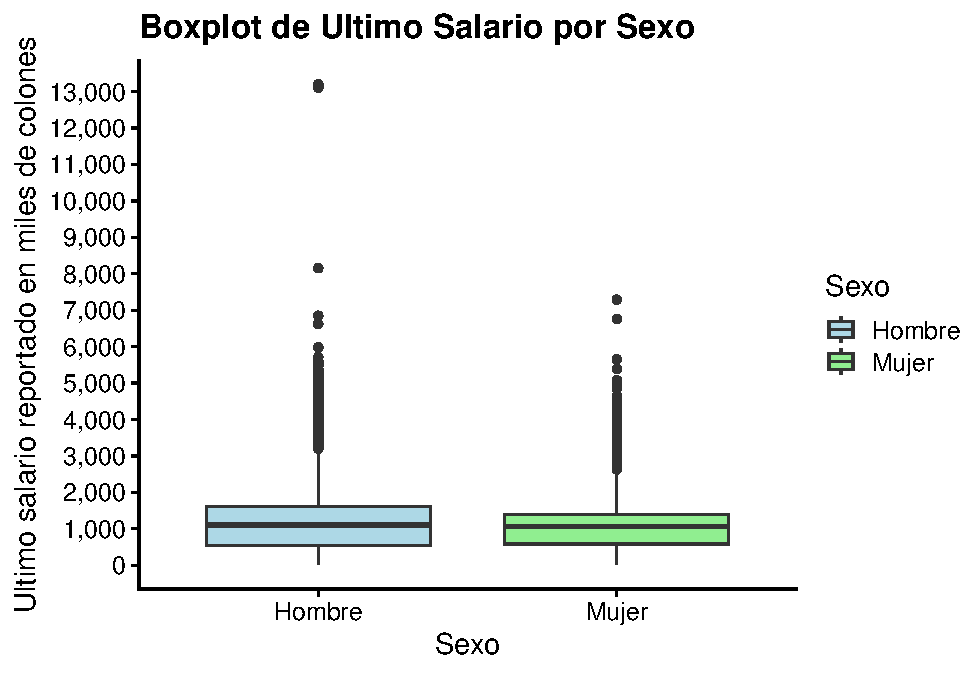
\includegraphics{Tarea1_files/figure-latex/unnamed-chunk-7-1.pdf}

Este gráfico destaca la presencia de salarios atípicos, identificados
como aquellos que están fuera de cada una de las cajas. Específicamente,
en el caso de los hombres, se observan dos salarios que se encuentran
notablemente por encima del resto de los salarios reportados, indicando
la presencia de valores atípicos significativos.

\hypertarget{conclusiones-con-respecto-a-los-salarios-y-sexo}{%
\subsection{Conclusiones con respecto a los salarios y
sexo}\label{conclusiones-con-respecto-a-los-salarios-y-sexo}}

Después de realizar el análisis descriptivo de los datos e interpretar
la gráfica de Boxplot, se concluye que al dividir la población por sexo,
el 25\% de los hombres con los salarios más bajos ganan menos que el
25\% de las mujeres con salarios más bajos. Sin embargo, cuando se
considera el 50\% de los hombres que ganan más, estos perciben un
salario mayor que el 50\% de las mujeres que ganan más. Esta tendencia
se evidencia claramente en el gráfico anterior, donde la parte superior
de la caja, que está por encima de la línea de la mediana, es más amplia
en el caso de los hombres.

Para respaldar este argumento, se observa que el promedio de los últimos
salarios fue mayor para los hombres, aproximadamente 110,540 colones más
alto que el de las mujeres.

No obstante, es importante señalar que la varianza de los salarios es
mayor para los hombres, y los valores atípicos en los salarios
masculinos también son más altos que los de las mujeres.

En este sentido, los salarios de los hombres parecen ser relativamente
más altos que los de las mujeres, aunque las diferencias no resultan
significativas. Ambos tienen personas con salarios más altos que la
mayoría.

\hypertarget{prueba-de-hipuxf3tesis-sobre-las-medias-de-las-categoruxedas-de-sexo}{%
\subsection{Prueba de hipótesis sobre las medias de las categorías de
sexo}\label{prueba-de-hipuxf3tesis-sobre-las-medias-de-las-categoruxedas-de-sexo}}

En relación a las medias, se cree que las medias de los salarios para
hombres y mujeres son diferentes. Para verificar lo expresado
anteriormente, se llevó a cabo la siguiente prueba de hipótesis.

En este caso, se llevó a cabo un \textbf{Welch Two Sample t-test}, la
cual es una prueba estadística que permite comparar las medias de dos
muestras. En este caso, el tamaño de las muestras y sus varianzas
difieren.

Para realizar una prueba de hipótesis se necesitan tres cosas: la
hipótesis nula (H0), el estadístico de prueba (t) y la distribución del
estadístico de prueba.

En este caso particular:

\begin{enumerate}
\def\labelenumi{\arabic{enumi}.}
\tightlist
\item
  H0: La diferencia entre la media de los últimos salarios de los
  hombres y la media de los últimos salarios de las mujeres es 0.
\item
  El estadístico de prueba es t, el cual se puede calcular de la
  siguiente manera:
  \[ t = \frac{\bar{X}_1 - \bar{X}_2}{\sqrt{\frac{s_1^2}{n_1} + \frac{s_2^2}{n_2}}} \]
  donde \(\bar{X}_1\) y \(\bar{X}_2\) son las medias de cada una de las
  muestras, \(s_1\) y \(s_2\) son las desviaciones estándar de los dos
  muestras, \(n_1\) y \(n_2\) son el tamaño de cada una de las muestras.
\item
  Por último, el estadístico t sigue una distribución t con \(v\) grados
  de libertad, la cual se calcula utilizando la equación
  Welch--Satterthwaite.
\end{enumerate}

A continuación se presenta el código de la prueba y la interpretación de
los resultados:

\begin{Shaded}
\begin{Highlighting}[]
\FunctionTok{t.test}\NormalTok{(}
  \AttributeTok{x           =}\NormalTok{ base\_salarios}\SpecialCharTok{$}\NormalTok{Ultimo.Salario[base\_salarios}\SpecialCharTok{$}\NormalTok{Sexo }\SpecialCharTok{==} \DecValTok{1}\NormalTok{],}
  \AttributeTok{y           =}\NormalTok{ base\_salarios}\SpecialCharTok{$}\NormalTok{Ultimo.Salario[base\_salarios}\SpecialCharTok{$}\NormalTok{Sexo }\SpecialCharTok{==} \DecValTok{2}\NormalTok{],}
  \AttributeTok{paired      =} \ConstantTok{FALSE}\NormalTok{,}
  \AttributeTok{alternative =} \StringTok{"two.sided"}\NormalTok{,}
  \AttributeTok{conf.level  =} \FloatTok{0.95}
\NormalTok{)}
\end{Highlighting}
\end{Shaded}

\begin{verbatim}
## 
##  Welch Two Sample t-test
## 
## data:  base_salarios$Ultimo.Salario[base_salarios$Sexo == 1] and base_salarios$Ultimo.Salario[base_salarios$Sexo == 2]
## t = 25.046, df = 49886, p-value < 0.00000000000000022
## alternative hypothesis: true difference in means is not equal to 0
## 95 percent confidence interval:
##  101889.5 119190.8
## sample estimates:
## mean of x mean of y 
##   1157202   1046661
\end{verbatim}

El p-valor lo que dice es si se asume la H0 como verdadera, la
probabilidad de que H0 sea verdadera. En este caso, el valor p fue menor
a \(2.2e^{16}\) lo cual es muy cercano a 0, es decir, hay una
probabilidad muy pequeña de que la media de los últimos salarios entre
hombres y mujeres sea 0, es decir, que sea la misma. Por tanto, existe
suficiente evidencia para rechazar la hipotesis nula.

\hypertarget{parte-ii}{%
\section{Parte II}\label{parte-ii}}

\hypertarget{construcciuxf3n-del-histograma-de-los-salarios}{%
\subsection{Construcción del Histograma de los
salarios}\label{construcciuxf3n-del-histograma-de-los-salarios}}

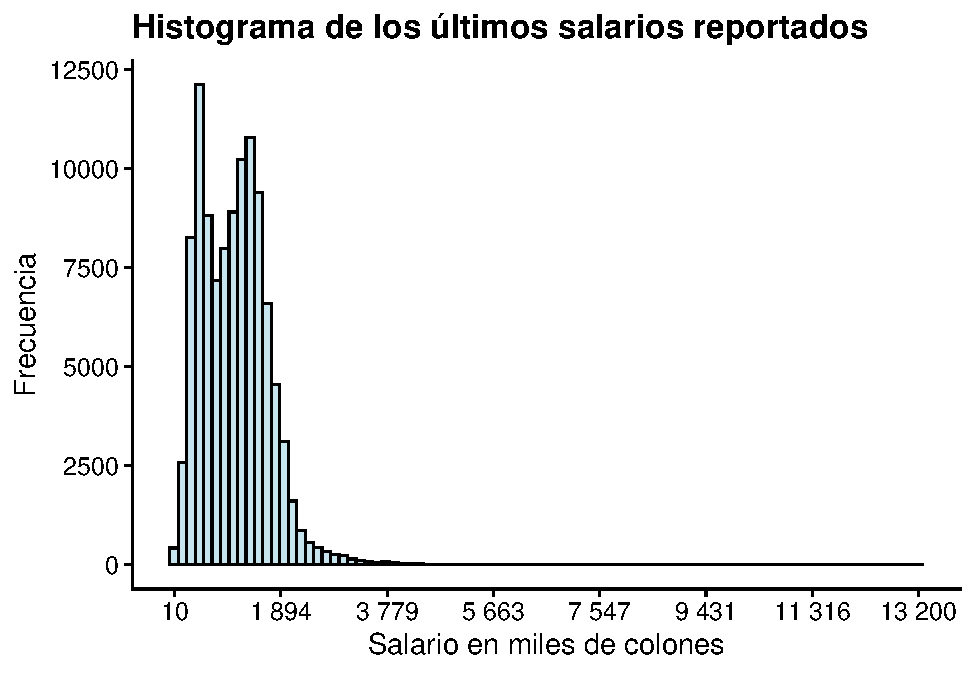
\includegraphics{Tarea1_files/figure-latex/unnamed-chunk-9-1.pdf}

\hypertarget{densidad-de-los-salarios-por-kernel-no-paramuxe9trica}{%
\subsection{Densidad de los salarios por kernel (no
paramétrica)}\label{densidad-de-los-salarios-por-kernel-no-paramuxe9trica}}

\hypertarget{densidad-de-los-salarios-por-kernel-usando-como-kernel-biweigth}{%
\subsubsection{Densidad de los salarios por kernel usando como kernel
Biweigth}\label{densidad-de-los-salarios-por-kernel-usando-como-kernel-biweigth}}

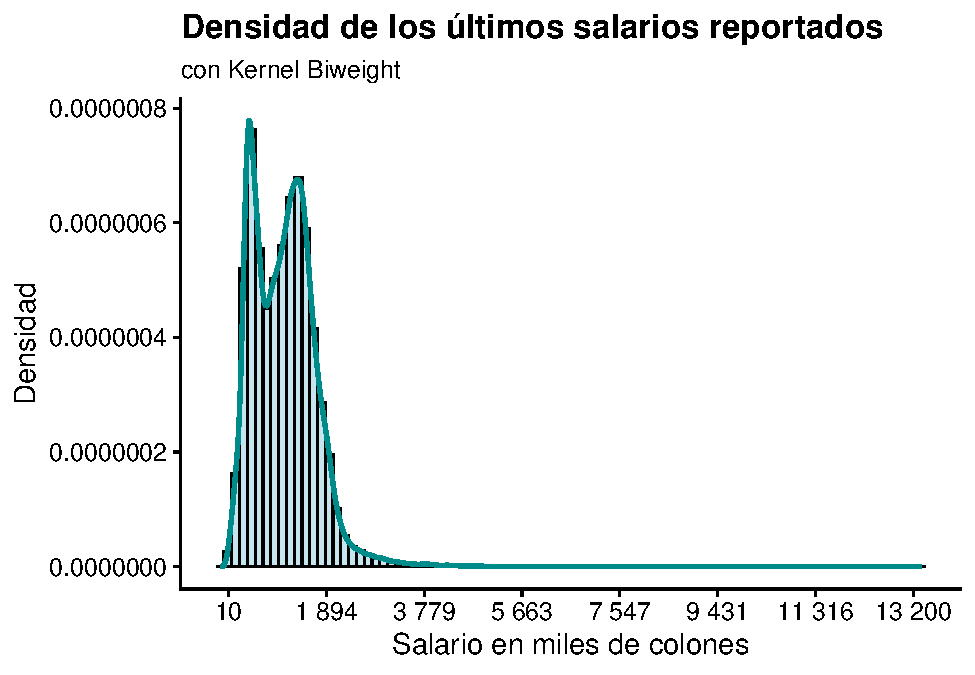
\includegraphics{Tarea1_files/figure-latex/unnamed-chunk-10-1.pdf}

\hypertarget{densidad-de-los-salarios-por-kernel-usando-como-kernel-normal}{%
\subsubsection{Densidad de los salarios por kernel usando como kernel
Normal}\label{densidad-de-los-salarios-por-kernel-usando-como-kernel-normal}}

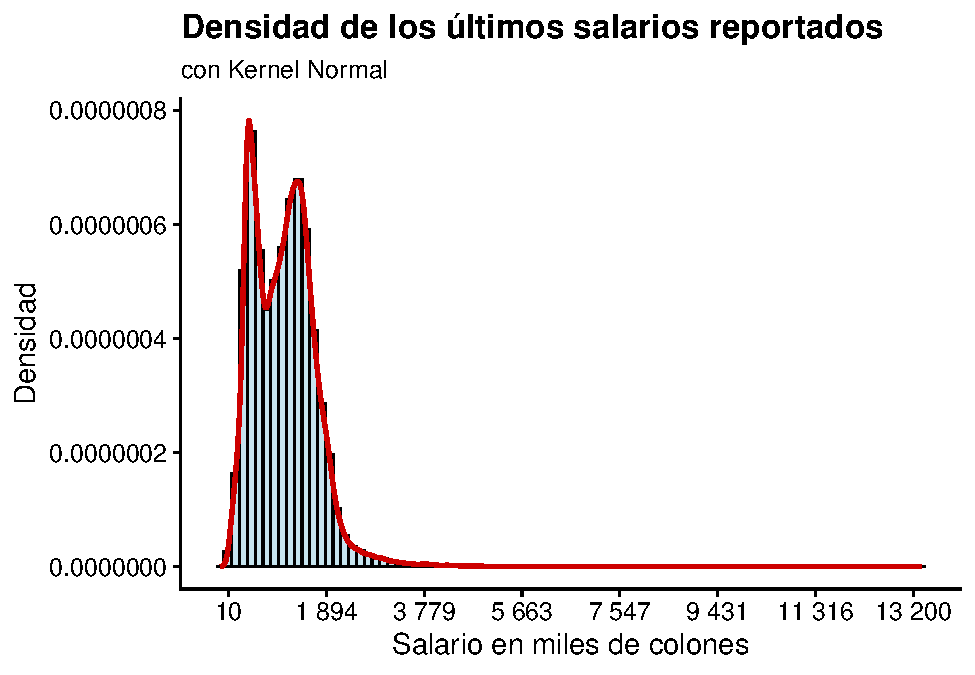
\includegraphics{Tarea1_files/figure-latex/unnamed-chunk-11-1.pdf}

\hypertarget{densidad-de-los-salarios-por-kernel-usando-como-kernel-epanechnikov}{%
\subsubsection{Densidad de los salarios por kernel usando como kernel
Epanechnikov}\label{densidad-de-los-salarios-por-kernel-usando-como-kernel-epanechnikov}}

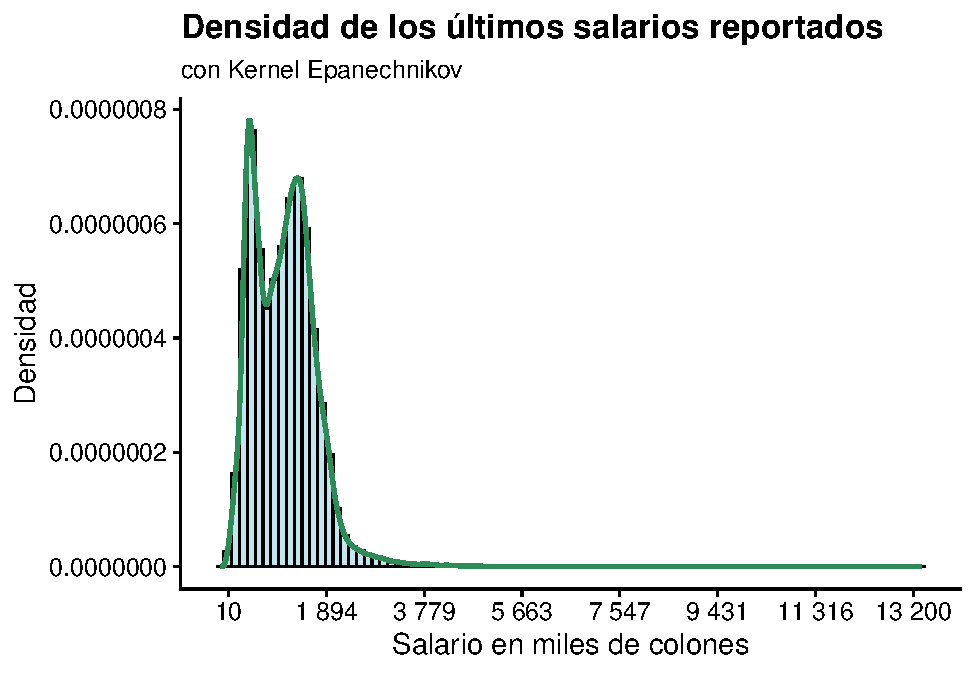
\includegraphics{Tarea1_files/figure-latex/unnamed-chunk-12-1.pdf}

\hypertarget{densidad-de-los-salarios-por-kernel-usando-como-kernel-coseno}{%
\subsubsection{Densidad de los salarios por kernel usando como kernel
Coseno}\label{densidad-de-los-salarios-por-kernel-usando-como-kernel-coseno}}

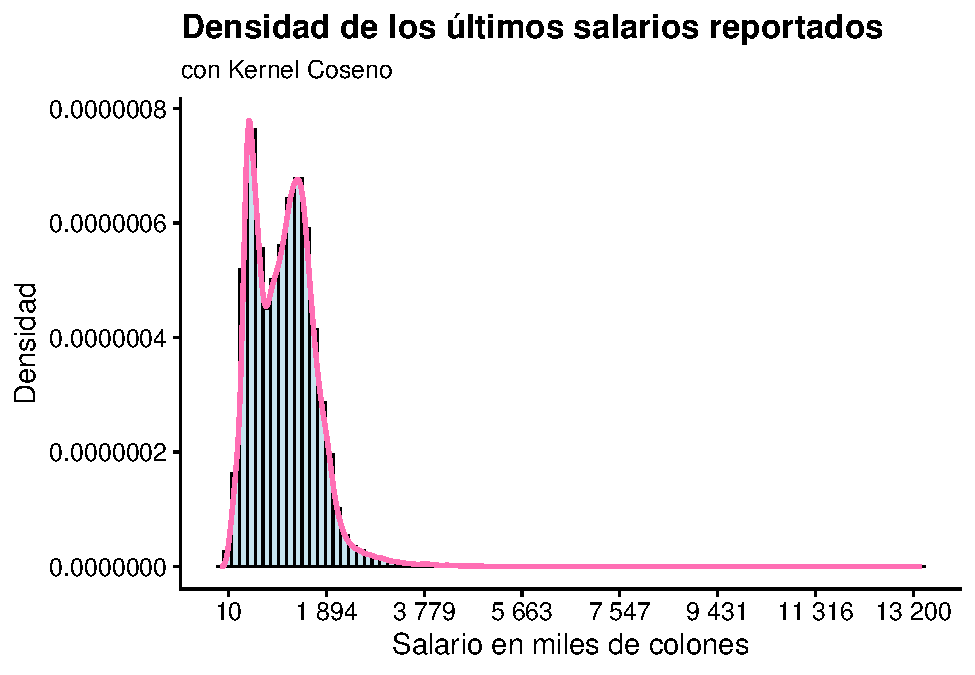
\includegraphics{Tarea1_files/figure-latex/unnamed-chunk-13-1.pdf}

\hypertarget{densidad-de-los-salarios-por-kernel-usando-como-kernel-rectangular}{%
\subsubsection{Densidad de los salarios por kernel usando como kernel
Rectangular}\label{densidad-de-los-salarios-por-kernel-usando-como-kernel-rectangular}}

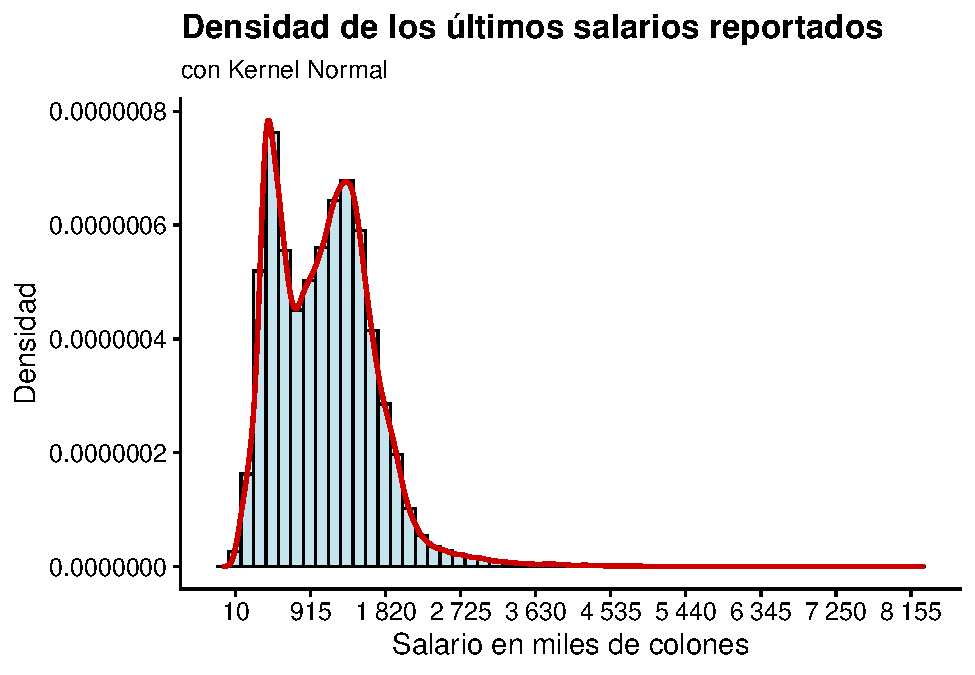
\includegraphics{Tarea1_files/figure-latex/unnamed-chunk-14-1.pdf}

\hypertarget{densidad-de-los-salarios-con-todos-los-kernel}{%
\subsubsection{Densidad de los salarios con todos los
kernel}\label{densidad-de-los-salarios-con-todos-los-kernel}}

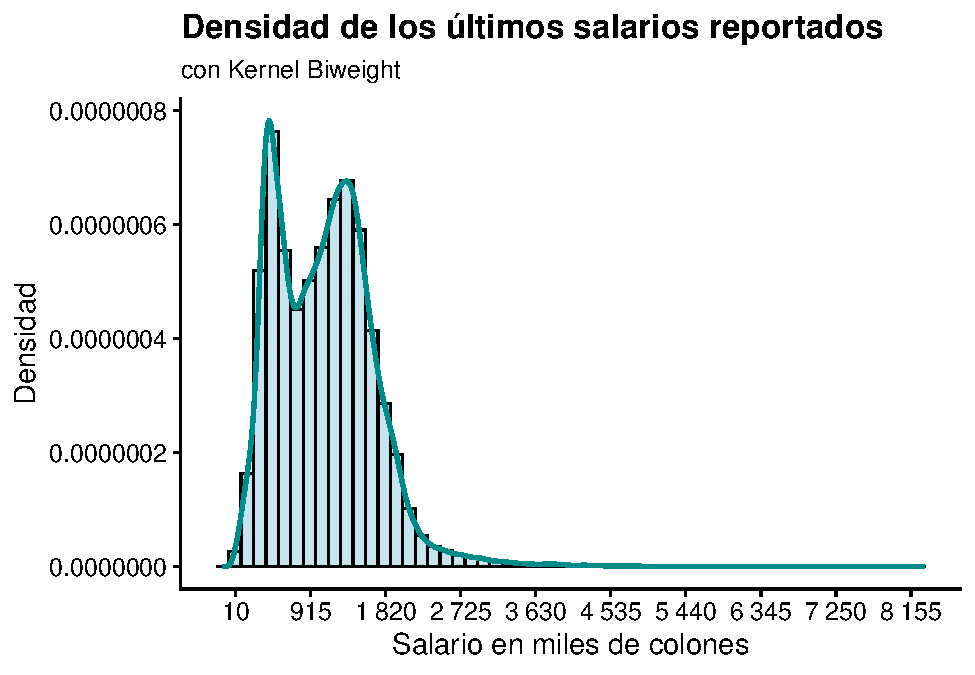
\includegraphics{Tarea1_files/figure-latex/unnamed-chunk-15-1.pdf}

\end{document}
